% a-project.tex, v-1.0.3 marcoreis baseado no
% abntex2-modelo-trabalho-academico.tex, v-1.9.7 laurocesar
% Copyright 2012-2018 by abnTeX2 group at http://www.abntex.net.br/ 
% 
% This work consists of the files 
% 
% -----------------------------------------------------------------------------
% Modelo para desenvolvimento de documentação de projetos acadêmicos
% (tese de doutorado, dissertação de mestrado e trabalhos de monografias em geral) 
% em conformidade com ABNT NBR 14724:2011: Informação e documentação. 
% -----------------------------------------------------------------------------
% Opções para a documentação
%
% Fancy page headings 
%\documentclass[fancyheadings, subook]{Classes/a-prj}
%\documentclass[fancyheadings, sureport]{Classes/a-prj}
%
% Fancy chapters and sections headings 
%\documentclass[fancychapter, subook]{Classes/a-prj}
%\documentclass[fancychapter, sureport]{Classes/a-prj}
%
% Fancy page , chapters and sections headings
%\documentclass[fancyheadings, fancychapter, subook]{Classes/a-prj}
\documentclass[fancyheadings, fancychapter, sureport]{Classes/a-report}
%
% -----------------------------------------------------------------------------
% Alguns comandos para a fancy page headings)
%
% Page header line width
%\footlinewidth{value}
%
% Page footer line width
%\headlinewidth{value}
%
% Page header and footer line width
%\headingslinewidth{value}
%
% Page header and footer lines without text
%\headingslinesonly
%
% The default line width is 0.3pt.
% Set the value to 0pt to remove the page header and/or footer line
%
% -------------------------------------------------------------------------------
% Formato de figuras suportado
% -------------------------------------------------------------------------------
% O formato das figuras depende da forma como o arquivo de saída é gerado.
% As figuras inseridas na pasta Figures serão automaticamente reconhecidas sem
% a necessidade de inserir a extensão do arquivo.
%
% O pdfLaTEX (PDF) suporta figuras com as extensões: pdf, jpg, png e mps.
%
% -------------------------------------------------------------------------------
% Árvore do diretório a-project.tex
%  Diretório
%       \Classes        (requerido)
%       \Figures        (requerido) --------------------------------->
%       \Figures\PDF    (optional)
%       \Figures\JPG    (optional) Figures located within these
%       \Figures\PNG    (optional) folders are searched automatically
%       \Figures\MPS    (optional)  by the a-prj class.
%       \Figures\EPS    (optional)
%       \Figures\PS     (optional) <--------------------------------
%       \Tables         (requerido)
%       \Others         (requerido)
%       \Chapters       (requerido)
%       \Appendices     (optional)
%       \References     (requerido)
%
% -------------------------------------------------------------------------------
% PDF File resumo
\ifpdf
    \hypersetup{
    	backref,
        colorlinks  = true,
        pdftitle    = Modelo de documentação,
        pdfauthor   = {Marco Reis, marco.a.reis@gmail.com},
        pdfsubject  = Mestre em Engenharia,
        pdfcreator  = Subtitulo,
        pdfproducer = PDFLatex,
        pdfkeywords = {documentação, latex, dissertação, tese}}
 \fi
%
% -------------------------------------------------------------------------------
% Relação de pacotes opcionais utilizados
\usepackage[utf8]{inputenc}
\usepackage[brazil]{babel}
\usepackage{longtable}
\usepackage{dcolumn}
\usepackage{multirow}
\usepackage{lscape}
%\usepackage{graphicx}
\usepackage{rotating}
%\usepackage{float,subfigure}
%\usepackage{graphicx, subfigure}
\usepackage{cite}
\usepackage[left=3cm,top=3cm,right=2cm,bottom=2cm]{geometry}
\usepackage[alf]{abntex2cite}
\usepackage{ifpdf}
\usepackage{shadow}
\usepackage{wrapfig}
\usepackage[normalem]{ulem}
\usepackage{makeidx}
\usepackage{yfonts}
\usepackage{algorithm}
\usepackage{algorithmic}
\usepackage{lmodern}
\usepackage[T1]{fontenc}
\usepackage{indentfirst}
\usepackage{color}
\usepackage{microtype}
\usepackage{lipsum}
\usepackage{caption}
\usepackage{subcaption}
\usepackage{ragged2e}
\justifying
%
\makeindex 
\setlength{\LTcapwidth}{\textwidth}
%
\newtheorem{theorem}{Teorema}
\newtheorem{definition}[theorem]{Definição}
%
% -------------------------------------------------------------------------------
% Configurações do pacote backref
\renewcommand{\backrefpagesname}{Citado na(s) página(s):~}
% Texto padrão antes do número das páginas
\renewcommand{\backref}{}
% Define os textos da citação
\renewcommand*{\backrefalt}[4]{
	\ifcase #1 %
		Nenhuma citação no texto.%
	\or
		Citado na página #2.%
	\else
		Citado #1 vezes nas páginas #2.%
	\fi
}
% 
% -------------------------------------------------------------------------------
% Início do documento raiz
\begin{document}
% Definição do título da página
    \university{Centro Universitário SENAI CIMATEC}
	%\faculty{Programa de...}
	%\school{Escola de...}
% 
    %\course{Engenharia Elétrica}
    % \typework{}
% 
	%\course{Mestrado em Modelagem Computacional e Tecnologia Industrial}
	%\typework{Disserta\c{c}\~ao de mestrado}
	%\typework{Exame de Qualificação de Mestrado}
% 
	%\course{Engenharia Elétrica}
	%\typework{Tese de doutorado}
	%\typework{Exame de Qualificação de doutorado}
%
% -------------------------------------------------------------------------------
% Informações gerais
    \thesistitle{Estudo do Estado da Arte:\\Quadrotores}
    \hidevolume
    \thesisvolume{Volume 1 of 1}
    \thesisauthorr{\:}
    \thesisauthor{Mateus Zarth Seixas}
    \thesisadvisor{Prof. Marco Reis, M.Eng.}
    %\hidecoadvisor
    %\thesiscoadvisor{Marco Reis}
    \thesismonthyear{Novembro de 2021}
% 
    \maketitlepage
%
% ----------------------------------------------------------------------------
% Inserir Folha de rosto, Nota de estilo, folha de assinaturas, dedicatoria
    \begin{folharosto}

\begin{center}
\theauthor \\
% \theauthorr \\
%\theauthorrr \\
%\theauthorrrr \\
%\theauthorrrrr \\
\end{center}
\ \\
\ \\
\ \\
\ \\
\ \\
\begin{spacing}{2}
   \begin{center}
   {\LARGE {\bf \thetitle}}
   \end{center}
\end{spacing}
\ \\
\ \\
\ \\
\vspace*{85mm}
% \begin{flushright}

%    \begin{list}{}{
%       \setlength{\leftmargin}{7.5cm}
%       \setlength{\rightmargin}{0cm}
%       \setlength{\labelwidth}{0pt}
%       \setlength{\labelsep}{\leftmargin}}

%       \item \thetypework apresentada ao \thefaculty, Curso de \thecourse
%       do \theuniversity, como requisito parcial para a obten\c{c}\~ao do
%       t\'itulo de {\bf \thedegreetitle}.

%       \begin{list}{}{
%       \setlength{\leftmargin}{0cm}
%       \setlength{\rightmargin}{0cm}
%       \setlength{\labelwidth}{0pt}
%       \setlength{\labelsep}{\leftmargin}}

%       \item \'Area de conhecimento: Interdisciplinar

%       \item Orientador: \theadvisor
%       \newline \hspace*{2.1cm}  %{\it \theuniversity}

%       \end{list}
%    \end{list}

% \end{flushright}
\ \\
\ \\
\ \\
\ \\
%\begin{spacing}{1.5}
   \begin{center}
   Salvador \par
   \theuniversity \par
   2021
   \end{center}
%\end{spacing}

\end{folharosto}

    %\begin{notaestilo}
Esta \thetypeworkthree foi elaborada considerando as normas de
estilo (i.e. est\'eticas e estruturais) propostas aprovadas pelo
colegiado do \thefacultytwo e est\~ao dispon\'iveis em formato
eletr\^onico ({\it download} na P\'agina Web
http:$//$ead.fieb.org.br$/$portal\_faculdades$/$dissertacoes-e-teses-mcti.html
ou solicita\c{c}\~ao via e-mail \`a secretaria do
programa) e em formato impresso somente para consulta. \\

Ressalta-se que o formato proposto considera diversos itens das
normas da Associa\c{c}\~ao Brasileira de Normas T\'ecnicas (ABNT),
entretanto opta-se, em alguns aspectos, seguir um estilo pr\'oprio
elaborado e amadurecido pelos professores do programa de
p\'os-gradua\c{c}\~ao supracitado.

\end{notaestilo}

    %\begin{folhaassinaturas}

%\thispagestyle{empty}

\def\signature#1#2{\parbox[b]{1in}{\smash{#1}\vskip12pt}
\hfill \parbox[t]{3in}{\shortstack{\vrule width 3in height
0.4pt\\\small#2}}}

\def\InstituicaoMembro#1#2{\parbox[b]{1in}{\smash{#1}\vskip12pt}
\hfill \parbox[t]{3in}{\shortstack{\vrule width 3in \\\small#2}}}

\def\signaturepage{%

    \begin{spacing}{1.5}
        \begin{center}
        {\LARGE \theuniversity} \\
        {\large \thefaculty} \\
        {\large \thecourse} \\
        \end{center}
    \end{spacing}

   \vskip 0.25in plus 0.4in minus 0.1in

    \begin{spacing}{1.5}
        \begin{sloppypar}
        A Banca Examinadora, constitu\'ida pelos professores abaixo
        listados, leram e recomendam a aprova\c{c}\~ao [com distin\c{c}\~ao] da
        \thetypeworktwo, intitulada ``\thetitle",
        apresentada no dia (dia) de (m\^es) de (ano), como requisito
        parcial para a obten\c{c}\~ao do t\'itulo de {\bf \thedegreetitle}.\\
        \end{sloppypar}
    \end{spacing}

    \def\sigskip{\vskip0.15in plus 0.2in minus 0.1in}
    \def\beginskip{\vskip0.3875in plus 0.2in minus 0.1in}

    \beginskip
    \signature{Orientador:}{Prof. Dr. \theadvisor} \\
    \InstituicaoMembro{}{\theuniversity} \\

    \sigskip
    \beginskip
    \signature{Membro externo da Banca:}{Prof. Dr. Nome completo} \\
    \InstituicaoMembro{}{Institui\c{c}\~ao do membro da banca} \\

    \sigskip
    \beginskip
    \signature{Membro externo da Banca:}{Prof. Dr. Nome completo} \\
    \InstituicaoMembro{}{Institui\c{c}\~ao do membro da banca} \\

    %\sigskip
    %\beginskip
   % \signature{Membro interno da Banca:}{Prof. Dr. Nome completo} \\
   % \InstituicaoMembro{}{Institui��o do membro da banca} \\

    \vfill
    \newpage
    \setcounter{page}{3}
}
%*********************************************************************


\signaturepage


\end{folhaassinaturas}

    %\include{Others/dedicatoria}
    %\include{Others/agradecimentos}
%
% ----------------------------------------------------------------------------
% Resumo/abstract, sumário e siglas
    % \begin{romanpagenumbers}
    %     \begin{thesisresumo}

Quadrotores são veículos aéreo não tripulados de asas rotativas que, por pussuírem diversas habilidades, vem se utilizados cada vez mais tanto para fins civís, como para fins militares. Este documeto traz o estudo do estado da arte (SOTA) sobre quadrotores, mostrando suas aplicações, classificações, opções de design, estudos sobre seus principais componentes, principais funcionalidades, como controle, planejamento de trajetória, localização e estudo sobre modelagem e identificação.

\ \\

% use de três a cinco palavras-chave

\textbf{Palavras-chave}: Palavra-chave 1, Palavra-chave 2, Palavra-chave 3, Palavra-chave 4, Palavra-chave 5

\end{thesisresumo}

    %     \begin{thesisabastract}
    Quadrotors are rotary-wing unmanned aerial vehicles that, due to their diverse abilities, are increasingly being used for both civil and military purposes. This document presents the state of the art (SOTA) of quadrotors, reviewing their applications,classifications, design options, studies on their main components, main features such as control, path planning, localization and study on modeling and identification.

\ \\

% use de tr�s a cinco palavras-chave

\textbf{Palavras-chave}: Quadrotors, State of the art, Review, unmanned aerial vehicles, SOTA

\end{thesisabastract}

    %     % Make list of contents, tables and figures
    %     \thesiscontents
    %     %\pdfbookmark[1]{Lista de Tabelas}{lot} \listoftables
    %     %\newpage
    %     %Include other required section
    %     %\begin{thesisabbreviations}
\begin{footnotesize}
\begin{longtable}[l]{p{2cm}l}
  tprax   \dotfill & \thefaculty \\
  WWW       \dotfill &  World Wide Web \\
\end{longtable}
\end{footnotesize}
\end{thesisabbreviations}

    %     %\begin{thesissymbols}
\begin{footnotesize}
\begin{longtable}[l]{p{2cm}l}
  $\partial$   \dotfill  & Bla bla bla \\
  $\prod$       \dotfill & ble ble ble \\
  $\partial$   \dotfill  & Bla bla bla \\
  $\prod$       \dotfill & ble ble ble \\
  $\partial$   \dotfill  & Bla bla bla \\
  $\prod$       \dotfill & ble ble ble \\
  $\partial$   \dotfill  & Bla bla bla \\
  $\prod$       \dotfill & ble ble ble \\
  $\partial$   \dotfill  & Bla bla bla \\
  $\prod$       \dotfill & ble ble ble \\
  $\partial$   \dotfill  & Bla bla bla \\
  $\prod$       \dotfill & ble ble ble \\
  $\partial$   \dotfill  & Bla bla bla \\
  $\prod$       \dotfill & ble ble ble \\
  $\partial$   \dotfill  & Bla bla bla \\
  $\prod$       \dotfill & ble ble ble \\
  $\partial$   \dotfill  & Bla bla bla \\
  $\prod$       \dotfill & ble ble ble \\
  $\partial$   \dotfill  & Bla bla bla \\
  $\prod$       \dotfill & ble ble ble \\
  $\partial$   \dotfill  & Bla bla bla \\
  $\prod$       \dotfill & ble ble ble \\
  $\partial$   \dotfill  & Bla bla bla \\
  $\prod$       \dotfill & ble ble ble \\
  $\partial$   \dotfill  & Bla bla bla \\
  $\prod$       \dotfill & ble ble ble \\
  $\partial$   \dotfill  & Bla bla bla \\
  $\prod$       \dotfill & ble ble ble \\
  $\partial$   \dotfill  & Bla bla bla \\
  $\prod$       \dotfill & ble ble ble \\
  $\partial$   \dotfill  & Bla bla bla \\
  $\prod$       \dotfill & ble ble ble \\
  $\partial$   \dotfill  & Bla bla bla \\
  $\prod$       \dotfill & ble ble ble \\
  $\partial$   \dotfill  & Bla bla bla \\
  $\prod$       \dotfill & ble ble ble \\
  $\partial$   \dotfill  & Bla bla bla \\
  $\prod$       \dotfill & ble ble ble \\          
\end{longtable}
\end{footnotesize}
\end{thesissymbols}

    %     %Switch the page numbering back to the default format
    % \end{romanpagenumbers}
%
% ---------------------------------------------------------------------------
% Include thesis chapters
    \parskip=\baselineskip
    \chapter{Introdução}
\label{chap:intro}

Este documento aborda o estudo do estado da arte de veículos aéreos não tripulados (VANTs) do tipo quadrotor, que são aeronaves de asas rotativas com quatro propulsores que podem se deslocar em todas as direções no espaço tridimensional. Esses veículos são comumentes chamados de Drones, que em inglês significa zangão ou zumbido, pelo barulho gerado pelos seus rotores em sua operação.

Os quadrotores são veículos muito ágeis, com grande manobrabilidade e payload, além de pussuírem a habilidade de realizar vôos estacionários e também pouso e decolagem vertical. Esses atributos tornam essas aeronaves muito úteis em diversas aplicações. Entretanto existem grandes desafios a serem enfrentados em sua operação, como controle, localização e autonomia.

Esta pesquisa apresenta os principais estudos acadêmicos realizados sobre este tipo de aeronave, principais autores, técnicas mais utilizadas aplicadas em suas funcionalidades e modelos já desenolvidos, para embasar o desenvolvimento de um projeto de concepção de um veículo dsse tipo.

%--------- NEW SECTION ----------------------
\section{Objetivos}
\label{sec:obj}

Este estudo foi realizado para dar suporte no denvolvimento de um quadrotor autônomo com capacidade de realizar pouso em uma plataforma móvel. Trazendo conhecimento das melhores técnicas que vem sendo utilizadas em áreas como navegação, controle e localização e mapeamento simultâneos (SLAM), assim como os melhores modelos e arquiteturas para conceber um veículo eficiente.

%--------- NEW SECTION ----------------------
\section{Justificativa}
\label{sec:justi}

Os VANTs tem sido cada vez mais utilizados para fins civís e militares. Tarefas que envolvem risco podem ser facilmente executadas por esse tipo de aeronave sem expor o piloto aos perigos associados a essa missão. Os drones tem sido utilizados em áreas como cinematografia, cartografia, vigilância, entrega de encomendas, mapeamento, entre outras. Devido a isso surge a importância de estudar essas aeronaves que apresentam alguns desafios a serem enfrentados como autonomia de vôo, localização e controle.

%--------- NEW SECTION ----------------------
\section{Organização do documento}
\label{section:organizacao}

Este documento apresenta $5$ capítulos e está estruturado da seguinte forma:

\begin{itemize}

  \item \textbf{Capítulo \ref{chap:intro} - Introdução}: Contextualiza o âmbito, no qual a pesquisa proposta está inserida. Apresenta, portanto, a definição do problema, objetivos e justificativas da pesquisa e como este \thetypeworkthree está estruturado;
  \item \textbf{Capítulo \ref{chap:fundteor} - Fundamentação Teórica}: XXX;
  \item \textbf{Capítulo \ref{chap:metod} - Materiais e Métodos}: XXX;
  \item \textbf{Capítulo \ref{chap:result} - Resultados}: XXX;
  \item \textbf{Capítulo \ref{chap:conc} - Conclusão}: Apresenta as conclusóes, contribuições e algumas sugestões de atividades de pesquisa a serem desenvolvidas no futuro.

\end{itemize}

    \chapter{Ambiente de Desenvolvimento}
\label{chap:ambiente}

\section{Ambiente de Aplicação}

Existem basicamente dois tipo de ambiente que os quadrotores aéreos podem atuar: o ambiente indoor e o ambiente outdoor. Nas missões em ambiente outdoor os quadrotores são expostos a ambientes desconhecidos, onde existe a forte presença de perturbações, como rajadas de vento e obstáculos dinâmicos. Nesse tipo de missão, os quadrotores muitas vezes vão precisar de sensores do tipo GPS para ajudar na localização do veículo e também, um controlador adequado para lidar com a rejeição de perturbação e com as incertezas paramétricas, além de um planejador de trajetória online. As missões indoor possuem menos perturbações e ambientes mais estruturados. Sendo possível fazer o mapeamento prévio do ambiente para realizar as operações.

\section{Situação Atual do Desenvolvimento}

As pesquisas mais atuais na área se concentram em áreas como controle, planejamento de trajetória, autonomia, percepção e navegação autônoma. O controle ainda é muito estudado pelo fato desse tipo de aeronave ser naturalmente instável, não-linear e subatuada, sendo necessário o desenvolvimento de controladores eficientes para realizar o segmento de trajetória, a rejeição de perturbação e ter insensibilidade a erros de modelagem e de incertezas paramétricas de forma ótima, com o menor gasto energético. O planejamento de trajetória também é desafiador pelo fato do ambiente de atuação ser tridimensional, que aumenta muito o custo computacional dos algoritmos. Isso torna necessário o estudo de algoritmos otimizados, com custos computacionais menores, permitindo que o planejador calcule trajetórias em tempos inferiores. Na questão de autonomia, uma grande limitação dos veículos aéreos de asas rotativas de forma geral é o gasto energético que a aeronave tem para manter vôo. Utilizar baterias maiores aumenta também o peso da aeronave, sendo necessário o estudo das melhores tecnologias que vem sendo usadas. Tem surgido pesquisas também de recarregamento desse tipo de aeronave wireless em estações preparadas para isso \cite{Mulgaonkar2014,Sierra2019,Abdilla2015b}. Para alcançar essas plataformas muitas vezes é necessário realizar um pouso autônomo,quesito que vem sendo muito estudado também em \cite{Lim2021,Simon2018,Falanga2017a,Jin2016a,Serra2016a,Kim2016,Ling2014,Serra2014,Herisse2012}.

\section{Mercado de Atuação}

O uso do veículos aéreos não tripulados do tipo quadrotor tem se expandido em diversas áreas, como civil, militar e acadêmica. Em aplicações militares, pelo fato desse tipo de aeronave possuir alta manobrabilidade e possibilidade de realizar vôos estacionários ou quase estacionários, eles podem ser utilizados em missões de espionagem, monitoramento e vigilância. Como elas não necessitam de um piloto embarcado, não colocando em risco o operador, e também por poderem ser muito pequenas, podem ser utilizadas em missão de busca e regaste em ambientes hostis, como em situações de desmoronamento. Na área civil, seu uso tem se popularizado muito para entretenimento, diversos modelos são comercializados com finalidade exclusivamente lúdica, sendo muitas vezes equipados com câmeras para captar imagens. Na área cinematográfica, tem sido utilizados para a realização de vídeos e fotografias aéreas, substituindo os helicópteros, que tinham custos associados maiores na sua operação. Seu uso tem se popularizado também na agricultura, para realização de monitoramento das plantações, irrigação agrícola, semeadura e distribuição de defensivos. Os quadrotor já tem sido utilizado até para a realização de entregas do tipo delivery, como mostrado na Figura \ref{fig:delivery}. No ambiente acadêmico, os quadrotores são utilizados como plataforma para teste de estratégias de controle, dada a dificuldade de se estabilizar e de controlar esse tipo de veículo, e também para teste de técnicas de planejamento de trajetória, pelo seu espaço de atuação ser tridimensional, o que torna as soluções mais complexas e com maior custo computacional.

\begin{figure} [h!]	
  \centering
  {
  \caption{Quadrotor Usado para Delivery}
  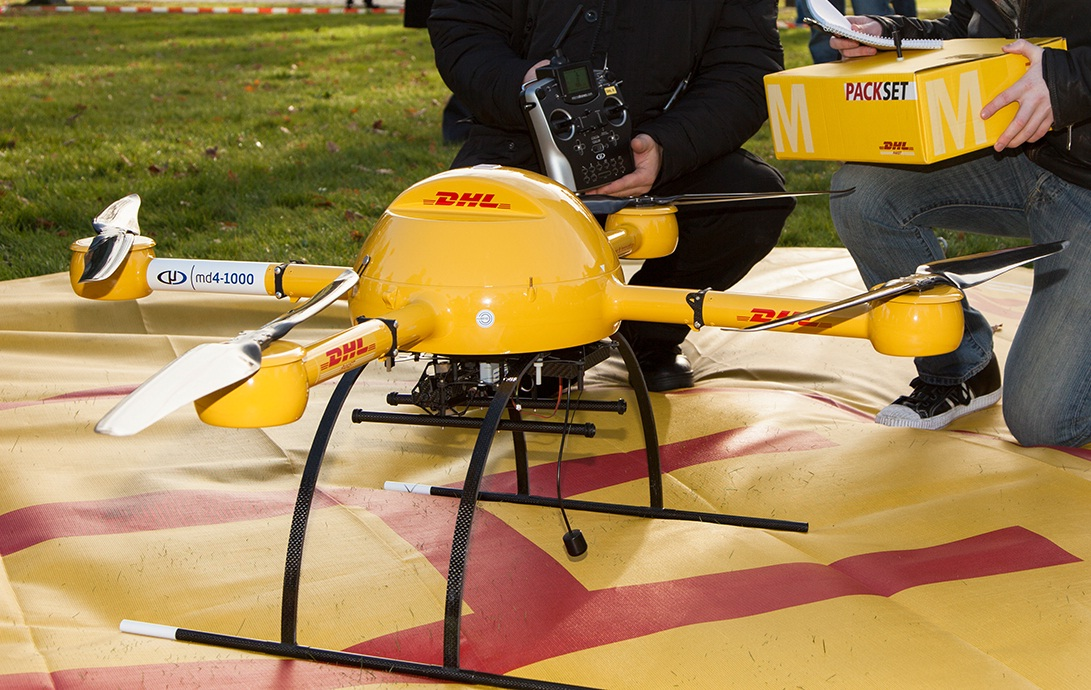
\includegraphics[width=0.7\textwidth]{Figures/Package_copter_microdrones_dhl.jpg}
  \caption*{Fonte:\url{https://upload.wikimedia.org/wikipedia/commons/0/0e/Package_copter_microdrones_dhl.jpg}}
  \label{fig:delivery}
  }
\end{figure}

\chapter{Metodologia}
\label{chap:metodologia}
%--------- NEW SECTION ----------------------
A pesquisa do estudo do estado da arte desenvolvida neste documento foi elaborada principalmente a partir do método BILI, que permite realizar uma pesquisa bibliográfica em um banco de dados de artigos científicos, publicações em periódicos, livros e outras fontes de conhecimento científicos, fazendo o levantamento das publicações e dos autores mais impactantes na área pesquisada. Também foram realizadas pesquisas para avaliar as soluções já encontradas no mercado.

O método BILI é dividido em quatro ciclos que acontecem em sequência. Eles são chamados de ciclo ingênuo, ciclo otimizada, ciclo de impacto e ciclo de produção.

% BIBLIOMETRIX


\begin{figure} [h!]	
  \centering
  \caption{Método BILI}
  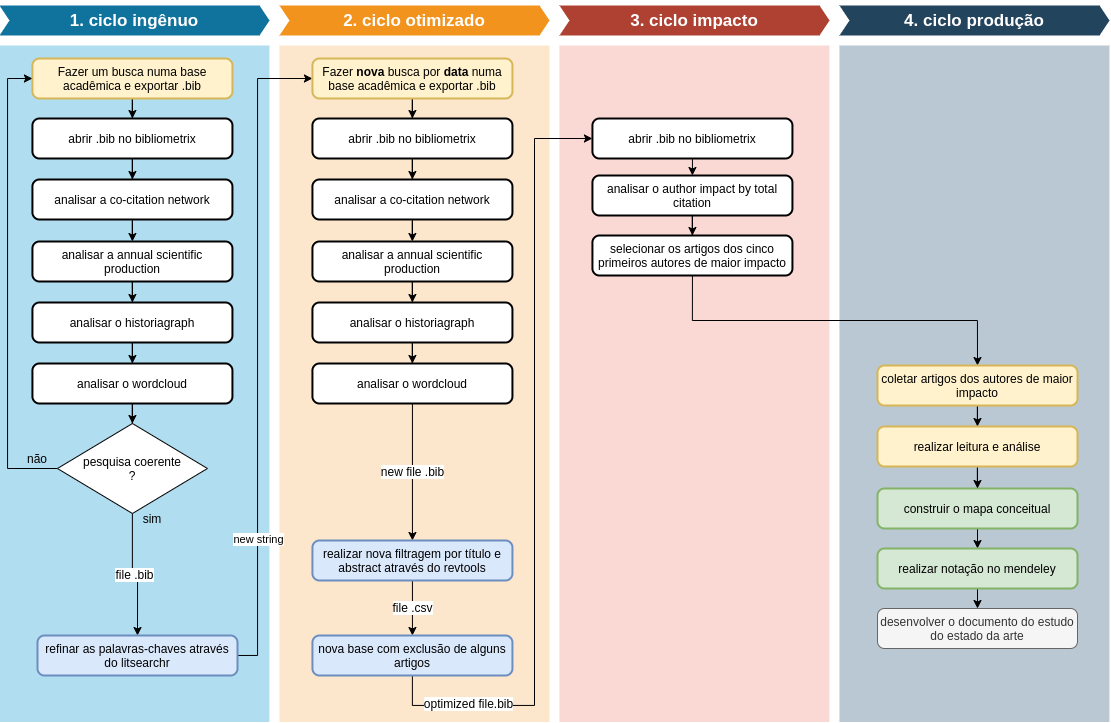
\includegraphics[width=1\textwidth]{Figures/bili.png}
  \caption*{Fonte: Autoria própria.}
  \label{fig:QFD}
\end{figure}

\section{Ciclo Ingênuo}
No primeiro ciclo do método BILI, é feita uma busca das pesquisas desenvolvidas na área estudada em um banco de dados de documentos acadêmicos através de palavras-chave que tenham conexão o tema proposto. O banco de dados escolhido para aplicar o método foi o Scopus.

O resultado da busca no banco de dados com as palavras-chave é um arquivo .bib, que contém o nome dos documentos encontrados, palavras-chave, ano de publicação, nome dos autores, DOI, resumo, entre outros.

Em seguida o arquivo .bib gerado no banco de dados é aberto no Bibliometrix, que é um pacote desenvolvido para R que permite uma clara visualização das informações levantadas e também realiza análises dos dados obtido. 

É então realizada a análise da rede de cocitação, que é um gráfico que relaciona os autores, mostrando a proximidade da pesquisa realizada por eles através de citações realizadas nas pesquisas. O resultado dessa análise é positivo se a rede de cocitação estiver coesa, com todos elementos conectados.

É avaliada também a produção científica anual, que é um gráfico que mostra quantas pesquisas foram realizadas na área pesquisada ao longo do tempo. O resultado desse gráfico é coerente quando se tem um crescimento positivo do número de pesquisas realizadas com o passar do tempo.

São avaliados por último os gráficos de histograph e wordcloud, que dão ideia das pesquisas mais importantes realizadas ao longo do tempo e das palavras-chave mais utilizadas, respectivamente.

Se a pesquisa não apresentar resultados coerentes, é realizada uma nova pesquisa com palavras-chave diferentes. Caso seja coerente, o próximo passo é fazer um refinamento das palavras-chave através do litsearchr, que é um pacote desenvolvido para R, que através do arquivo .bib obtido, fornece as palavras-chave mais impactantes dos dados.

\section{Ciclo Otimizado}
Com as palavras-chave otimizadas obtidas através do litsearchr, é feita uma nova busca no banco de dados acadêmico escolhido, no caso o Scopus, para obter um novo arquivo .bib, da mesma forma que foi obtido no primeiro ciclo.

Os gráfico de rede de cocitação, produção científica anual, wordcloud e histograph são analisados novamente, para avaliar a coerência. Caso verificada a coerência do resultado, é realizada uma filtragem dos resultados através do revtools. O revtools é um pacote desenvolvido também para R que possibilita a realização da leitura do resumos das pesquisas e é possível manter a pesquisa caso ela seja útil ou excluir caso ela não sirva.

O resultado do revtools é um arquivo .csv contendo apenas os documentos que são úteis para a pesquisa. O arquivo então é convertido novamente para o formato .bib e então passado para o próximo ciclo.

\section{Ciclo de Impacto}
O arquivo .bib gerado no ciclo anterior é novamente aberto no Bibliometrix. Nessa etapa é avaliado o gráfico de author impact by total citation e levantados de três a cinco autores com maior impacto apresentados no gráfico.

\section{Ciclo de Produção}
Por último são coletados os artigos dos autores selecionados no banco de dados e é feita a leitura completa dos artigos. 

É feito o upload dos artigos e leitura na plataforma Mendeley. Nesse aplicativo é possível compartilhar os artigos com grupos de estudo, fazer anotações e grifar trechos importantes. 

A partir dos conhecimentos adquiridos é feito um mapa conceitual que relaciona os principais conceitos apresentados para servir de base para o desenvolvimento desse documento.
    \chapter{Estudo do Estado da Arte}
\label{chap:metod}
Nessa pesquisa foram abordados diversos aspectos que envolvem a concepção de um projeto envolvelmento um UAV do tipo quadrotor. O desenvolvimento de uma plataforma desse tipo ainda envolve desafios estruturais, autonomia, controle, localização entre outros, que necessitam de estudo prévio detalhado para ser alcançado um bom resultado com o veículo.

% %--------- NEW SECTION ----------------------
\section{Quadrotores}
% \label{sec:ui}
Quadrotores são aeronaves de asas rotativas, ou seja, são sustentandas e movimentadas por rotores. Diferente das aeronaves de asas fixas, como aviões, os aeronaves de asas rotativas não utilizam seu movimento horizontal para sustentar seu vôo. Isso faz com que esse tipo de veículo apresente um consumo energético muito maior. Apesar disso, as aeronaves de asas rotativas possuem a habilidade de realizar pouso e decolagem vertical, além de poder realizar vôos estacionários.

As aeronaves de asas rotativas são classificadas como multirotores, sendo seus tipos mais importantes quadrotores, hexarotores, octarotores, coaxiais ou helicópteros. Os quadrotores são veículos que apresentam alta manobrabilidade e alto payload, mas apresentam também alto gasto energético, tornando baixa o seu tempo de vôo, sendo um desafio achar baterias mais efieciente que aumentem sua autonomia. A medida que aumenta-se o número de rotores, passando de quadrotores para hexarotores e octarotores, aumenta-se também o payload, que é o quanto a aeronave consegue carregar em relação ao seu peso, e a tolerância a falha, que é continuar realizando um vôo controlado mesmo com algumas das hélices apresentando falhas de funcionamento. Entretanto, diminui-se também a manobrabilidade e aumenta-se o consumo energético.

\subsection{Classificações}
Os quadrotores são classificados em diversas categorias, possuindo cada uma delas caracacterísticas específicas, que podem ajudar no design do projeto e também na escolha de componentes que vão ajudar na operação da aeronave.

\subsubsection{Classificação Quanto ao Peso}
Os UAVs são classificados em diversas categorias de acordo com o quanto eles pesam. UAVs que pesam até 2 quilogramas (kg) são classificados como micro, de 2 kg até 7 kg são classificados como mini, de 7 kg até 25 kg são classificados como pequenos, de 25 kg até 150 kg, como médios e de 150 kg em diante são classificados como grandes.\\
Quadrotores mais leves são mais ágeis por serem menores e por isso terem inércias menores. Possuindo assim maiores. acelerações angulares 

\subsubsection{Classificação Quanto a Configuração}
Os quadrotores tem duas configurações possíveis em relação à disposição de seus rotores. Os rotores podem ter a a configração em forma de "+", em que a frente da aeronave fica alinhada com uma das hastes que suporta um par de rotores. Essa configuração também é conhecida como cruz. A outra confuração possível é a configuração em "x", em que a frente da aeronave fica a 45$^{\circ}$ do eixo que contém a haste da aeronave, ficando assim a frente da aeronave no meio de duas hastes, como mostrado na Figura.

A configuração em "+" é mais acrobática, entretando, como desvantagens, a haste dos rotores bloqueia o campo de visão da câmera e também apresenta um momento de guinada ao translacionar, necessitando de um maior gasto energético para estabilizar a aeronave.

A configuração em "x" não apresenta esse efeito, por ter os movimentos de arfagem e rolagem desacoplados do de guinada. Apresenta menor esforço para transladar pois todos rotores agem nesses movimentos, diferente da configuração em "+", em que apenas um par de rotores é responsável pelo deslocamento enquanto o outro se mantém com velocidades constantes. É mais estável, entrentando apresenta menor manobrabilidade.

\subsubsection{Ambiente de Operação}
Os quadrotores podem operar em dois tipos de missões: outdoor e indoor. As missões outdoor são as missões em que os quadrotores são expostos a ambientes desconhecidos, onde existe a forte presença de pertubações, como rajadas de vento. Nesse tipo de missão, os quadrotores muitas vezes vão precisar de sensores do tipo GPS para ajudar na localização do veículo e também de um controlador adequado para lidar com a rejeição de pertubação. As missões indoor possuem menos pertubações e ambientes mias estruturados. Sendo possível fazer o mapeamento prévio do ambiente para realizar as operações 

\subsection{Principais Componentes}

\subsubsection{Sensores Inerciais}

Os VANTs são geralmente equipados com uma IMU (Inertial Measurement Unit), que são dispositos que são compostos por giroscópios, acelerômetros e magnetômetros. Os giroscópios são sensores capazes de medir a velocidade angular do veículo nos três eixos, os acelerômetros são responsáveis por calcular as acelerações lineares nos três eixos e o magnetômetro mede campos magnéticos nos três eixos. Devido ao forte campo magnético existente no planeta Terra, é possível obter a orientação do robô também através da obtenção da magnitude do campo magnético atuando no eixos da aeronave. Através da fusão sensorial é possível obter a atitude do robô e realizar odometria. Muita vezes também são utilizdos sensores do tipo barômetro, que são sensores capazes de medir a pressão atmosférica. Como a pressão atmosférica varia com a altitude, é possível mensurar a altura da aeronave em relação ao nível do mar da aeronave com a utilização desse sensor.

\subsubsection{Motores}

Falar sobre hélices?

Os motores DC são máquinas elétricas de corrente contínua (CC) que são constituídos por uma armadura ou rotor que é a parte giratória montada sobre o eixo da máquina, um estator de material ferromagnetico envolvido pelo enrolamento de campo, um comutador com função de manter o torque gerado em um determinado sentido e de escovas, que são conectores fixos que permitem od eslizamento do comutador no eixo da armadura. enrolamento de armadura. Os motores DC possuem uma grande variabilidadade de velocidade de operação, podendo operar acima e abaixo do valor nominal, possuem alta aceleração, podendo varias de velocidade rapidamente, inclusive mantendo o toqrque constante e não necessitam de conversores complexos. Como desvantagens, eles necessitam de manutenção constante para a troca de escovas, são mais caros e maiores do que motores CA com mesma potência e também possuem centelhamento.

O motor brushless DC (BLDC) é um motor de corrente contínua síncrono que é alimentado por corrente contínua (CC) e não possui escovas de contato elétrico. Ele é composto por imãs permanentes, chamados de magnetos, que podem ser localizados no estator externo ou no centro no estator interno. A vantagem desse tipo de motor é que eles são altamente eficientes, pois possuem menos perdas por atrito, resultando em torques maiores. Essa eficiência é de grande valia para os quadrotores, pois um grande desafio associado a operação com esse tipo de veículo é a autonomia. A redução do atrito também faz com que a vida útil desse tipo de motor seja maior e que seja necessário ter menos manutenções, por não necessitar trocar as escovas.

\subsubsection{Baterias}

Um grande desafio a ser enfrentado no trabalho com veículos áereos de asas rotativas é a autonomia. Graças ao grande gasto energético que essas aeronaves possuem para se sustentar no ar o tempo de vôo desses veículos acaba se tornando baixo.   

As baterias mais amplamente utilizadas para UAVs são baterias polímero de lítio (LiPo). Esse tipo de bateria tem uma das melhores relações entre capacidade e peso, o que é de vital importância para esse tipo de veículo, já que o peso das baterias é algo em torno de 50\% do peso da aeronave. As baterias LiPo possuem uma capacidade regular e um bom ciclo de vida. Em (Abdilla, 2015) é feito um estudo do consumo de energia de multirrotores e uma modelagem para estimação da autonomia do veículo operando com baterias LiPo.  

\subsubsection{Microprocessador}

\section{Revisão Bibliográfica}
% \label{sec:ui}
\subsection{Autores}
\subsection{Artigos}

\section{Ambiente de Aplicação}
% \label{sec:ui}
O uso do veículos aéreos não tripulados do tipo quadrotor tem se expandido em diversas áreas, tanto civíl, quanto militar e também acadêmica.

No ambiente acadêmico, os quadrotores são utilziados como plataforma para teste de estratégias de controle, dada a dificuldade de se estabilizar e de controlar esse tipo de veículo, e também para teste de técnicas de planejamento de trajetória, por se deslocar no espaço tridimensional.

Os quadrotores por não necessitarem de um piloto embarcado, poderem ser pequenos e ágeis podem ser utilizados em missões de busca e resgate em abientes hostis, como casos de desmoronamento ou soterramento, e também em missões de espionagem e vigilância, por chamaerem pouca atenção.

Tem-se crescido muito o uso de aeronaves do tipo quadrotor na área de agricultura de precisão. Os drones podem ser utilizados para monitorar uma lavroura, mapear, distribuir uso de defensivos, semear e até mesmo irrigar.

Outra área de grande utilização é a de enterterimento. Existem muitos drones são comercializados com finalidade exclusivamente lúdica, podendo ser equipados com câmeras para produzir fotografias e vídeos. São utilizados tambpem na cinematografia para realizar essas filmagnes aéreas, que antes eram feitas por helicópteros tripulados que tinham custo associados muito maiores.


\section{Funcionalidades}
% \label{sec:ui}

\subsection{Modelagem}
A modelagem de um quadrotor é uma das etapas mais importantes no desenvolvimento de um projeto envolvendo esse tipo de veículo. Por ser uma plataforma instável, se torna inviável realizar técnicas de identificação em malha aberta. Sendo assim, é necessário obter o modelo dinâmico da aeronave através de técnicas de modelagem.

A modelagem da aeronave pode ser obtida através das equações de Newton-Euler ou através do formalismo de Euler-Lagrange (CASTILLO 2005). Através dessa modelagem é possível obter o modelo de alto nível, onde os torques e forças são entradas e as saídas são posições angulares e lineares. 

\subsection{Controle}
Os quadrotores são veículos subatuadas, ou seja, possuem mais graus de liberdade do que atuadores, são naturalmente instáveis e apresentam comportamento não-linear. Devido a esses fatores, esse tipo de veículo necessita de uma estrutura de controle adequada bem ajustada para que sejá possível a estabilização e o seguimento de referência.

Os controladores que atuam no quadrotor geralmente são utilizados em cascata (NONAMI,2010), de forma que existe um controle de baixo nível para garantir uma velocidade de rotação desejada nos rotores, um controlador em um npivel mais alto para controlar a altitude e as velocidade angulares de rolagem, arfagem e rolagem e por último um controlador no nível mais alto controladando posições lineares no espaço tridimensional. (kendoul)

Controlador hierárquico, estabilidade global

Os controlador mais comumente usado em baixo nível para controlar a velocidade de de roatação dos propulsores é o PID. 

Os controladores que controlam atitude, altitude e posições lineares no quadrotor podem ser controladores lineares ou não-lineares. Para serem utilizados controladores lineares é necessário realizar uma linearização do modelo matemático do quadrotor, considerando pequenas variações de ângulo. Os controladores lineares que são mais amplamente utilizados são os controladores PID, LQR, H2, H$\infty$ e controle adaptativo. Como alguns parãmetros do quadrotor podem apresentar incertezas ou até mesmo variar durante a operação, também é possível adcionar robustez a esses controladores, podendo ajudar também na rejeição de pertubação.

Os controladores não-lineares mais amplamente utilizados são os controladores por inversão de modelo, o sliding mode control (SMC) e o controlador Fuzzy.

\subsection{Localização}
A localização do quadrotor pode ser auxiliada por uso de diversos sensores como LiDAR, GPS, IMU, câmeras monoculares, sensores ultrassônicos e lasers.

A IMU pode ser utilizada para a funcionalidade de localização através da odometria. A IMU pode contar com giroscópio, acelerômetro, magnetômetro e até mesmo barômetro.

Os sensores que são mais amplamente utilizados atualmente são os sensores baseados em visão. É possível obter bons resultados apenas utilizando câmeras monoculares, como mostrado em ... utilizando o pacote ORB Slam.

Os sensores GPS são amplamente utilizados para missões outdoor e os sensores ultrassônicos e baseados em laser são utilizados para auxiliar na medição da altitude.

Pode-se realizar a fusão sensorial de diversos sensores para se obter uma boa estimativa da localização da aeronave. A técnica mais amplamente utilizada é a de filtragem, como a do filtro extendido de kalman, EKF, porém ela sofre com o drift, que é um deslocamento não considerado pela medição. Outra opção é o ? framework de otimização não-linear, que apresenta resultados mais consistentes, porém apresenta um custo computacional superior.

\subsection{Planejamento de Trajetória}
O planejamento de trajetória é fundamental para que o quadrotor se torne uma plataforma completamente autônoma. Através dessa funcionalidade o veículo pode calcular uma rota para se deslocar da sua posição atual até uma posição final sem a interferência humana, sendo de extrema importância para o objetivo final do projeto que é tornal o drone capaz de realizar um pouso autônomo em uma plataforma móvel.

Diversas técnicas de planejamento de trajetória tem sido usados para lidar com o problema Belief Rodamap (onde eu vi?), A*, algorítmos? genéticos, e algorítmoos com inteligência artificial

Em (v. Roberge 2013) (smiluação) foi feito um estudo de comparação entre o planejamento de trajeoria através do algoritmo genético e da otimização por enxame de partículas. explicar as técnicas.
Ambas as técnicas aprtesentaram boas soluções em tempos computacionais relativamente curtos (quanto?). Como conclusão foi observado que com significância estatística o GA apresenta melhores trajetórias ao PSO. Para comparar os resultados foi realizar o t-teste sobre o a função custo

Em (Y CHEM,2014) é feito o planejamento de trajetória através da técnica Artificial Potential Field, que é vantajosa por ser implementada através de um algoritmo de estrutura simples, com uma descrição matemática conscistente e conveniente para controle em tempo real, além de possuir uma grande portabilidade, podendo solucionar o problema de desvio de obstáculos mundando a fonte do campo potencial artificial. (Y CHEM,2014). A técnica também pode ser utilizada para o planejamento de trajetória de vôo em formações de múltiplos UAVs. Apesar das diversas vantagens, o APF na configuração padrão não resulta na trajetória ótima, sendo possível ser combinado com outras técnicas como o algoritmo genético ou algoritmos evolucionários para melhorar seus resultados. FALAR de NMPC? O APF é baseado na idéia de que o destino funciona como um campo potencial atrativo para o UAV, enquanto os obstáculos funcionam como campos potenciais repulsivos. Nessa pesquisa, o APF é reconstruído sobre a otimização com restrições introduzida com a força de controle adicional.

Em (Y Chem,2015), é utilizada um algoritmo de de otimização derivado do Central Force Optimizatin (CFO), chamado de Modified Central Force Optimization. O CFO é um algoritmo de otimização de partícula inteligente baseado na lei da gravidade, onde cada solução é uma partícula. As partículas se atraem com a força gravitacional virtual. As massas dessas partículas são dependendes da função custo de cada solução. Na metáfora do CFO, quando uma massa está sobre forte influência de uma massa, ela fica presa em seu campo gravitacional, o que é análogo a localizar um valor máximo para uma função objetivo.
No MCFO são adcionados conceitos da otimização por Enxame de partículas (PSO) além do operador de mutação do algoritmo genético (GA) para melhorar os resultados do CFO. Os resultados da poesquisa mostraram resultados em simulação superiores aos das técnicas com o algoritmo CFO, GA, PSO e de bucas aleatórias. FA? tambem.

Em (muller 2015), é apresentado um método computacional mente eficiente que calcula trajetórias com funções de posição polinomiais três vezes diferenciáveis, considerando as retrições de velocida e aceleração do veículo. O algoritmo foi testado com a captura de uma bola arremessada pelo quadrotor.
 
\begin{itemize}
    \item Artificial potential field
    \item probabilistic roadmap
    \item belief roadmap
    \item potential fields (PF)
    \item Heuristic search algorithms
    \item Optimization methods
    \item planning under uncertainties
    \item reactive and bio-inspired obstacle avoidance methods
\end{itemize}



\section{Mapa Conceitual}
% \label{sec:ui}
    \chapter{Resultados}
\label{chap:result}
Importante sempre ter um parágrafo introdutório para explicar os resultados encontrados.

%--------- NEW SECTION ----------------------
\section{Testes unitários}
\label{sec:testu}
\lipsum[1]

\section{Integração do sistema}
\label{sec:intsis}
\lipsum[1]

%--------- NEW SECTION ----------------------
\section{Testes integrados}
\label{sec:testi}
\lipsum[1]








    \chapter{Conclusão}
\label{chap:conc}

Chegou a hora de apresentar o apanhado geral sobre o trabalho de
pesquisa feito, no qual s\~ao sintetizadas uma s\'erie de
reflex\~oes sobre a metodologia usada, sobre os achados e
resultados obtidos, sobre a confirma\c{c}\~ao ou recha\c{c}o da
hip\'otese estabelecida e sobre outros aspectos da pesquisa que
s\~ao importantes para validar o trabalho. Recomenda-se n\~ao
citar outros autores, pois a conclus\~ao \'e do pesquisador.
Por\'em, caso necess\'ario, conv\'em cit\'a-lo(s) nesta parte e
n\~ao na se\c{c}\~ao seguinte chamada \textbf{Conclus\~oes}.


\section{Considerações finais}
\label{sec:consid}

Brevemente comentada no texto acima, nesta se\c{c}\~ao o
pesquisador (i.e. autor principal do trabalho cient\'ifico) deve
apresentar sua opini\~ao com respeito \`a pesquisa e suas
implica\c{c}\~oes. Descrever os impactos (i.e.
tecnol\'ogicos,sociais, econ\^omicos, culturais, ambientais,
políticos, etc.) que a pesquisa causa. N\~ao se recomenda citar
outros autores.


    % include more chapters ...
%
% ----------------------------------------------------------------------------
% Include thesis appendices
    \begin{thesisappendices}
        % Thesis Appendix -------------------------------------------------------

\chapter{Diagramas mecânicos}
\label{Append:diagmec}



        % Thesis Appendix -------------------------------------------------------

\chapter{Diagramas eletro-eletrônicos}
\label{Append:diagele}



        %% Thesis Appendix -------------------------------------------------------

\chapter{Logbook}
\label{Append:log}



    \end{thesisappendices}
%
% ----------------------------------------------------------------------------
% Configurar as referencias bibliograficas
	\renewcommand\bibname{Referências}
    \addcontentsline{toc}{chapter}{Referências}
    \bibliography{References/referencias}
%
% ----------------------------------------------------------------------------
% Finishing him
    \include{Others/ultimafolha}
\end{document}
%
% -------------------------------------------------------------------------------
% Aqui termina a formatação para o documento.
% In God We Trust. All Other Bring Data. 
%
% -------------------------------------------------------------------------------